\documentclass[a4paper, oneside, 12pt]{article}
\usepackage[utf8]{inputenc}

\title{Verjetnost 2}
\author{vesna.irsic }
\date{January 2016}

\usepackage[slovene]{babel}
\usepackage[utf8]{inputenc}
\usepackage[T1]{fontenc}
\usepackage{url}
\usepackage{graphicx}
\usepackage[usenames]{color}
\usepackage[reqno]{amsmath}
\usepackage{amssymb, amsthm}
\usepackage{enumerate}
\usepackage{array}
\usepackage{titlesec}
\usepackage[bookmarks, colorlinks=true, %
linkcolor=black, anchorcolor=black, citecolor=black, filecolor=black, %
menucolor=black, runcolor=black, urlcolor=black%
]{hyperref}
\usepackage[
    paper=a4paper,
    top=1cm,
    bottom=1cm,
%    textheight=24cm,
    textwidth=19cm,
    ]{geometry}

\usepackage{icomma}
\usepackage{units}

\newtheorem{izrek}{Izrek}
\newtheorem{posledica}{Posledica}

\theoremstyle{definition}
\newtheorem{definicija}{Definicija}
\newtheorem{opomba}{Opomba}
\newtheorem{zgled}{Zgled}

\def\R{\mathbb{R}}
\def\N{\mathbb{N}}
\def\Z{\mathbb{Z}}
\def\C{\mathbb{C}}
\def\Q{\mathbb{Q}}
\def\multiset#1#2{\ensuremath{\left(\kern-.3em\left(\genfrac{}{}{0pt}{}{#1}{#2}\right)\kern-.3em\right)}}

% lists with less vertical space
\newenvironment{itemize*}{\vspace{-10pt}\begin{itemize}\setlength{\itemsep}{0pt}\setlength{\parskip}{2pt}}{\end{itemize}}
\newenvironment{enumerate*}{\vspace{-10pt}\begin{enumerate}\setlength{\itemsep}{0pt}\setlength{\parskip}{2pt}}{\end{enumerate}}
\newenvironment{description*}{\vspace{-12pt}\begin{description}\setlength{\itemsep}{0pt}\setlength{\parskip}{2pt}}{\end{description}}

\setlength{\parindent}{0pt}
\setlength{\parskip}{8pt}

\titleformat*{\section}{\large\bfseries}
\titleformat*{\subsection}{\large\bfseries}
\titleformat*{\subsubsection}{\bfseries}
\titlespacing*{\section}{0pt}{6pt}{-1pt}   % left, before, after
\titlespacing*{\subsection}{0pt}{6pt}{-1pt}

\newcommand{\dd}[2]{\ensuremath{\frac{\partial #1}{\partial #2}}}
\newcommand{\dt}[1][]{\dd{#1}{t}}
\newcommand{\dx}[1][]{\dd{#1}{x}}
\newcommand{\dy}[1][]{\dd{#1}{y}}
\newcommand{\dz}[1][]{\dd{#1}{z}}
\newcommand{\dth}[1][]{\dd{#1}{\theta}}
\newcommand{\dphi}[1][]{\dd{#1}{\phi}}
\renewcommand{\H}{\ensuremath{\hat{H}}}

\renewcommand{\b}{\boldsymbol}

\usepackage{bbold}
\newcommand{\ind}{\ensuremath{\mathbb{1}}}
\newcommand{\indset}[1]{\ind_{\{\text{#1}\}}}

\begin{document}
\pagestyle{empty}

\section*{Bernik part}
\textbf{Markovske verige v diskretnem času:}\\
Markovska veriga z 2 stanjema:
$P = \begin{bmatrix}
1-a & a  \\
b & 1-b\end{bmatrix}$,
$P^n = \frac{1}{a+b}
\begin{bmatrix} b+ a \lambda_2^n & a-a \lambda_2^n \\
b-b\lambda_2^n & a+ b \lambda_2^n \end{bmatrix}$, \\
lastni vrednosti $P$: $\lambda_1 = 1, \lambda_2 = 1-a-b$.
(sled matrike je enaka vsoti lastnih vrednosti)\\
Pri računanju pogojnih verjetnosti:\\
- uporabljaj lastnost Markova (zgodovina ni pomembna)\\
- uporabljaj homogenost verige (če je vseeno, kje začneš)\\
- po potrebi združiš stanja, narediš kakšno stanje absorbirajoče \ldots \\
- razbijanje na bloke (če rabiš povprečno št. korakov, da se nekaj zgodi npr.)\\
- $(P^n)_{i,j} = P(X_n = j | X_0 = i)$; namesto potenciranja matrike lahko pošičeš lastne vrednosti $P$: \\$ P(X_n=j | X_0=i) = \pi_j \cdot 1^n + B \cdot \lambda_2^n + \ldots$, konstante dobiš, ko vstaviš $n = 0, 1, \ldots$\\
- variacije na temo $P(A|B) = \frac{P(A \cap B)}{P(B)}$\\
- Bayesova formula $P(A|B)=\frac{P(B|A) P(A)}{P(B)}$; $P(A,B|C) = \frac{P(C|A,B)P(A,B)}{P(C)} = \frac{P(B,C|A)P(A)}{P(C)}$\\
- izpeljanke: $P(A|B\cap C) = P(B|A,C)\frac{P(A|C)}{P(B|C)}$, $P(A|B) = P(D|B) P(A| B,D) + P(D^c|B) P(A|B,D^c)$\\
Če iščeš stacionarno porazdelitev:\\
- Jordanska forma, poiščeš $\lim_{n \to \infty} P^n$ (vse vrstice v limitni matriki so levi lastni vektor za lastno vrednost 1)\\
- poiščeš levi lastni vektor k lastni vrednosti $1$: $\pi = \pi P$, $\pi$ je vrstica\\
- poiščeš kakšne rekurzivne zveze in rešiš sistem diferenčnih enačb (nastavek $\lambda^n$) -- gledaš kaj je prvi korak\\
Če je matrika dvojno stohastična, je $\pi = [ 1/N, \ldots, 1/N]$, kjer je $N$ število stanj.\\
Če za vse $i,j$ velja $p_{ij} \pi_i = \pi_{ji} \pi_j$, je $\pi$ stacionarna porazdelitev.\\
$\tilde{T}_x = \inf \{n \geq 1 \; ; \; X_n = x\}$ čas zadetja.\\
Za ireducibilno markovsko verigo, ki ima stacionarno porazdelitev
($\iff$ obstaja pozitivno povrnljivo stanje $\iff$ vsa stanja so pozitivno povrnljiva)
velja $\pi_x = \frac{1}{E_x[\tilde{T}_x]}$. Obratno, če želiš pričakovani čas ponovne vrnitve v
$x$: $E_x[\tilde{T}_x] = \frac{1}{\pi_x}$. Povprečno število obiskov stanja $i$ gre v verjetnosti proti $\pi_i$. Če je veriga aperiodična (npr.\ graf ni 2-delen), je $P_{ij}(n) \to \pi_j$, če je periodična s periodo $d$ je $P_{ij}(nd + r) \to d \pi_j$.\\
$\rho_{xy} = P_x[\tilde{T_y} < \infty]$. Stanje je povrnljivo, če $\rho_{xx} = 1$, minljivo, če $\rho_{xy} < 1$. Pozitivno povrnljivo, če $E_x[\tilde{T_x}] < \infty$, ničelno povrnlivo, če $E_x[\tilde{T_x}] = \infty$.\\
Če imamo $P_1, P_2$ prehodni matriki in na vsakem koraku vržemo kovanec ($P(\text{grb}) = p$); če pade grb, se premaknemo v skladu s $P_1$, sicer v skladu s $P_2$. Dobimo markovsko verigo s prehodno matriko $P = p P_1 + (1-p) P_2$.\\
$P$ je $m\times m$ markovska veriga in $Q$ je $n \times n$ markovska veriga, različna stanja, neodvisni.Tudi $(X_i, Y_i)$ je markovska veriga, prehodna matrika je $P \otimes Q$, tj.\ $(P \otimes Q_{(i,j), (k,l)}) = P_{ik} Q_{jl}$.\\
Isto kot zgoraj. Na vsakem koraku vržemo kovanec, ki pove, katera veriga se premakne, druga veriga ostane v istem stanju. Tudi to je markovska veriga. Če $K_1, K_2, \ldots$ zaporedje metov kovancev in $S_n = K_1 + \cdots + K_n$, je $n$-to stanje te verige $R_n = (X_{S_n}, Y_{n-S_n})$.\\
$P$ prehodna matrika markovske verige, $i$ stanje: $f_i = P_i(X_n = i \text{ za nek } n \geq 1)$, $N_i = $ število obiskov v $i = \sum_{n=0}^\infty \mathbb{1}_{\{X_n = i\}}$. Velja $E_i[N_i] = \sum_n (P^n)_{i i} = 1 + \frac{1}{1-f_i}$.\\
Simetričen slučajen sprehod v $\Z^d$: $0$ je povrnljivo stanje le za $d = 1, 2$.\\
Če imamo graf, kjer je prehodna verjetnost enakomerna $p_{ij} = \frac{1}{\deg(i)} \ind(i\sim j)$,
potem je stacionarna porazdelitev reverzibilna in velja
$\pi_i = \frac{\deg(i)}{\sum \deg(j)} = \frac{\deg(i)}{2E}$.\\
Če imamo naključne nize iz 0 in 1 z verjetnostjo $p$ za 1 in nas zanima $E[\emptyset \to 1010]$. Potem rečemo:
$E[\emptyset \to 1010] = E[\emptyset \to 10] + E[10 \to 1010] = E[10 \to 10] + E[1010\to 1010] =
\frac{1}{\pi_{10}} + \frac{1}{\pi_{1010}} = \frac{1}{p(1-p)} + \frac{1}{p^2(1-p)^2}$.
Vedno razbijemo tako, da pogledamo najdaljši suffix, ki je tudi prefix in
nadaljujemo od tega suffixa naprej.
Če nas zanima verjetnost, da se nek niz pojavi pred drugim, potem naredimo tako: označimo s $K$ število korakov,
ki jih rabimo da vidimo $X$ in $Y$. Velja:
$E[K] = E[\emptyset \to X] + P(X \text{ pred } Y)E[X \to Y] =
E[\emptyset \to Y] + P(Y \text{ pred } X)E[Y \to X]$.
Iz te enačbe lahko izračunamo $P(X \text{ pred } Y)$.\\
Stirling: $n! \sim n^n e^{-n} \sqrt{2\pi n}$.\\ \\

\textbf{Markovske verige v zveznem času:}
Imamo generator $G$ z intenzitetami $\lambda_{ij}$. Digaonalni element je obratno predznačena vsota vseh ostalih.
Intenziteta $\lambda_{ij}$ pove, kako se spreminja verjetnost, da bomo skočili iz $i$ v $j$
($\lambda_{ii} < 0$, torej verjetnost, da ostanemo v $i$ pada -- porazdelitev $exp(\lambda_{ii})$).\\
Če označimo $P_{ij}(t) = P(X_t = j|X_0 = i)$, potem veljata naprejšnja in nazajšnja enačba Kolmogorova:
$\dot{P}(t) = GP(t)$ in $\dot{P} = PG(t)$. Rešitev: $P(t) = e^{Gt}$. Velja tudi $P(X_t = i | X_0 = i) = 1 - \lambda_{ii} t + o(t^2), P(X_t = j | X_0 = i) = \lambda_{ij} t + o(t^2)$.\\
Lahko rešuje z rodovnimi funkcijami. Napišemo $P_{ij}'(t) = \sum_{k} P_{ik}(t)G_{kj}$,
pomnožimo z $s^j$ in seštejemo po $j$. Dobimo PDE za funkcijo $F_i(t, s) = \sum_{j=0}^{\infty} P_{ij}(t)s^j$. (Če rešuješ s separacijo, je splošna rešitef $f(r(s,t))$, če $r$ tvoja rešitev in $f$ poljubna.)
PDE rešimo in razvijemo v vrsto po $s$, preberemo verjetnosti.\\
Uporabno: $(1+x)^n = \sum_{k=0}^{\infty} \binom{n}{k}x^n$\\
Stacionarna porazdelitev $\pi$ je levi lastni vektor za lastno vrednost $0$, da ga dobimo rešimo
enačbe $\pi G = 0$.\\
Hitting time: $T_i^+=\inf\{t>0; X_t=i, X_{t^-}\neq i\}$; velja $E_i[T_i^+]=\frac{1}{\pi_i \lambda_{ii}}$.\\
Z dvema stanjema:
$G = \begin{bmatrix} -\alpha & \alpha\\ \beta & -\beta \end{bmatrix}$,
$P(t) = \frac{1}{\alpha+\beta} \begin{bmatrix}
  \beta + \alpha e^{-(\alpha+\beta)t} & \alpha - \alpha e^{-(\alpha+\beta)t} \\
  \beta - \beta e^{-(\alpha+\beta)t} & \alpha + \beta e^{-(\alpha+\beta)t} \end{bmatrix}$,
  $\pi = [\frac{\beta}{\alpha + \beta}, \frac{\alpha}{\alpha+\beta}]$\\
  Neodvisni markovski verigi $X$, $Y$, z generatorjema
  $G = \begin{bmatrix} -a & a\\ b & -b \end{bmatrix}$ in
  $G = \begin{bmatrix} -c & c\\ d & -d \end{bmatrix}$ dobimo markovsko verigo $(X,Y)$ z generatorjem
  $GH = \begin{bmatrix} - (a+c)& c & a & 0\\ d & -(a+d) & 0 & a \\ b & 0 & -(b+c) & c
  \\ 0 & b & d & -(b+d) \end{bmatrix}$, $\pi = \frac{1}{(a+b)(c+d)}[bd, bc, ad, ac]$.

\section*{Stoyanov part}
\textbf{Moments:} $X$ rv. $k$-th moment: $E[X^k]$. \\
MGF -- moment generating function $M_X(t) = E[e^{tX}] = \sum_{k=0}^\infty \frac{E[X^k]}{k!} t^k$. \\
$E[X^k] = \frac{d^k M_X}{dt^k}(0)$.
Moment generating functions are positive and log-convex, with $M(0) = 1$. \\
Strong Cramer condition: $M(t)<\infty, \forall t \in \mathbb{R}$;
Cramer condition: $M(t)<\infty, \forall t \in [0,t_0); t_0 > 0$ fixed.\\
If $X \sim F$, existing m.g.f. $M(t), t \in (-t_0, t_0), t_0 > 0$: (1.) All moments of $X$ are finite: $m_k = E(X^k) < \infty$ and moreover, $m_k =M^{(k)}(0)$ (2.) F is the only d.f. with the moment seq. ${m_k, k = 1,2, \dots}$ (F is M-determinate)\\
\textbf{Characteristic function:} $\psi_X(t) = E[e^{itX}]$ (Fourier transform).
Velja: $\psi_X(-it) = M_X(t)$. \\
The characteristic function of a real-valued random variable always exists and
is uniformly continuous on the entire space. $\psi_X(0) = 1$, $|\psi_X(t)| \leq 1$.
If $|\psi_X(t)| = 1$ for some $t \neq 0$, then $X$ is discrete.
If $|\psi_X(t)| = 1$ for some $t \in (a, b)$, then $X$ is almost surely constant.
$\psi_X(-t) = \psi_X(t)$. In particular, the characteristic function of a symmetric
random variable is real-valued and even.
$X$ and $Y$ both have the same distribution iff $\psi_{X}=\psi_{Y}$.
$E[X^k] = (-i)^k \psi_X^{(k)}(0)$.
If $X_1, \ldots, X_n$ are independent, and $a_1,\ldots, a_n \in \C$
then $\psi_{a_1X_1+\cdots+a_nX_n}(t) = \psi_{X_1}(a_1t)\cdots \psi_{X_n}(a_nt)$. \\
Inversion formula (finding $F$): $a<b$ points of continuity of $F$; $F(b)-F(a) = \lim_{T\rightarrow \infty}\frac{1}{2}\int_{-T}^{T}\frac{e^{-itb}-e^{-ita}}{-it}\psi(t)dt$\\
Inverse Fourier transform (for absolutely continuous case $f=F'$): $f(x) = \frac{1}{2 \pi}\int_{-\infty}^{\infty} e^{-itx}\psi(t)dt$\\
Trik: $\psi_{XY}(t) = E[\psi_Y(tX)] = E[\psi_X(tY)]$.\\
\textbf{Log-Normal:}
$Z \sim N(0,1)$, $Y = \exp(Z) \Rightarrow Y \sim \operatorname{Log}N(0,1)$. $F_Y(x) = \Phi (\ln x)$, $f(x) = 1/\sqrt{2\pi}\cdot 1/x\cdot \exp(-1/2\cdot(\ln x)^2)$ where $x > 0, f(x) = 0$ for $x \leq 0$. Heavy tail, no m.g.f.. It's not the only dist. with the moments $(\exp(k^2/2), k=1,2,..)$ Importance: B-S model\\
\textbf{Tipi konvergence:}
In distribution: $(X_n) \to X \sim F$ as $n \to \infty$ if $F_n(x) \to F(x)$ as $n \to \infty$. In probability: if $P(|X_n - X| \leq \epsilon) \to 1$. In space $L^r$: if $E(|X_n -X|^r) \to 0$ Properties: If in $L^r$ $\Rightarrow$ in prob. $\Rightarrow$ in distr.\\
\textbf{Transforms $\boldsymbol{Y=g(X)}$:} $g$ increasing on range of $X$: $F_Y(y)=F_X(g^{-1}(y))$,
$f_Y(y)=f_X(g^{-1}(y))\frac{d}{dy}g^{-1}(y)$;\\
$g$ decreasing on range of $X$: $F_Y(y)=1-F_X(g^{-1}(y))$, $f_Y(y)=f_X(g^{-1}(y))|\frac{d}{dy}g^{-1}(y)|$.\\
Vsota: $f_{X + Y} (x) = \int f(x-y) g(y) dy = \int g(x-y) f(y) dy$\\
\textbf{Inequalities:}
Chebyshev: (assume $X \in L^2$) $P(|X -E(X)| > \epsilon) \leq Var(x)/ \epsilon^2 $;
Markov: (X non neg.) $P(X\geq a) \leq \frac{E(X)}{a}$; Jensen: $X$, $g$ convex, $0<s<r$: $(E[|X|^s])^{1/s} \leq (E[|X|^r])^{1/r}$.

% čast in hvala moji sestri, ker je to prepisala :) Wow, hvala :)
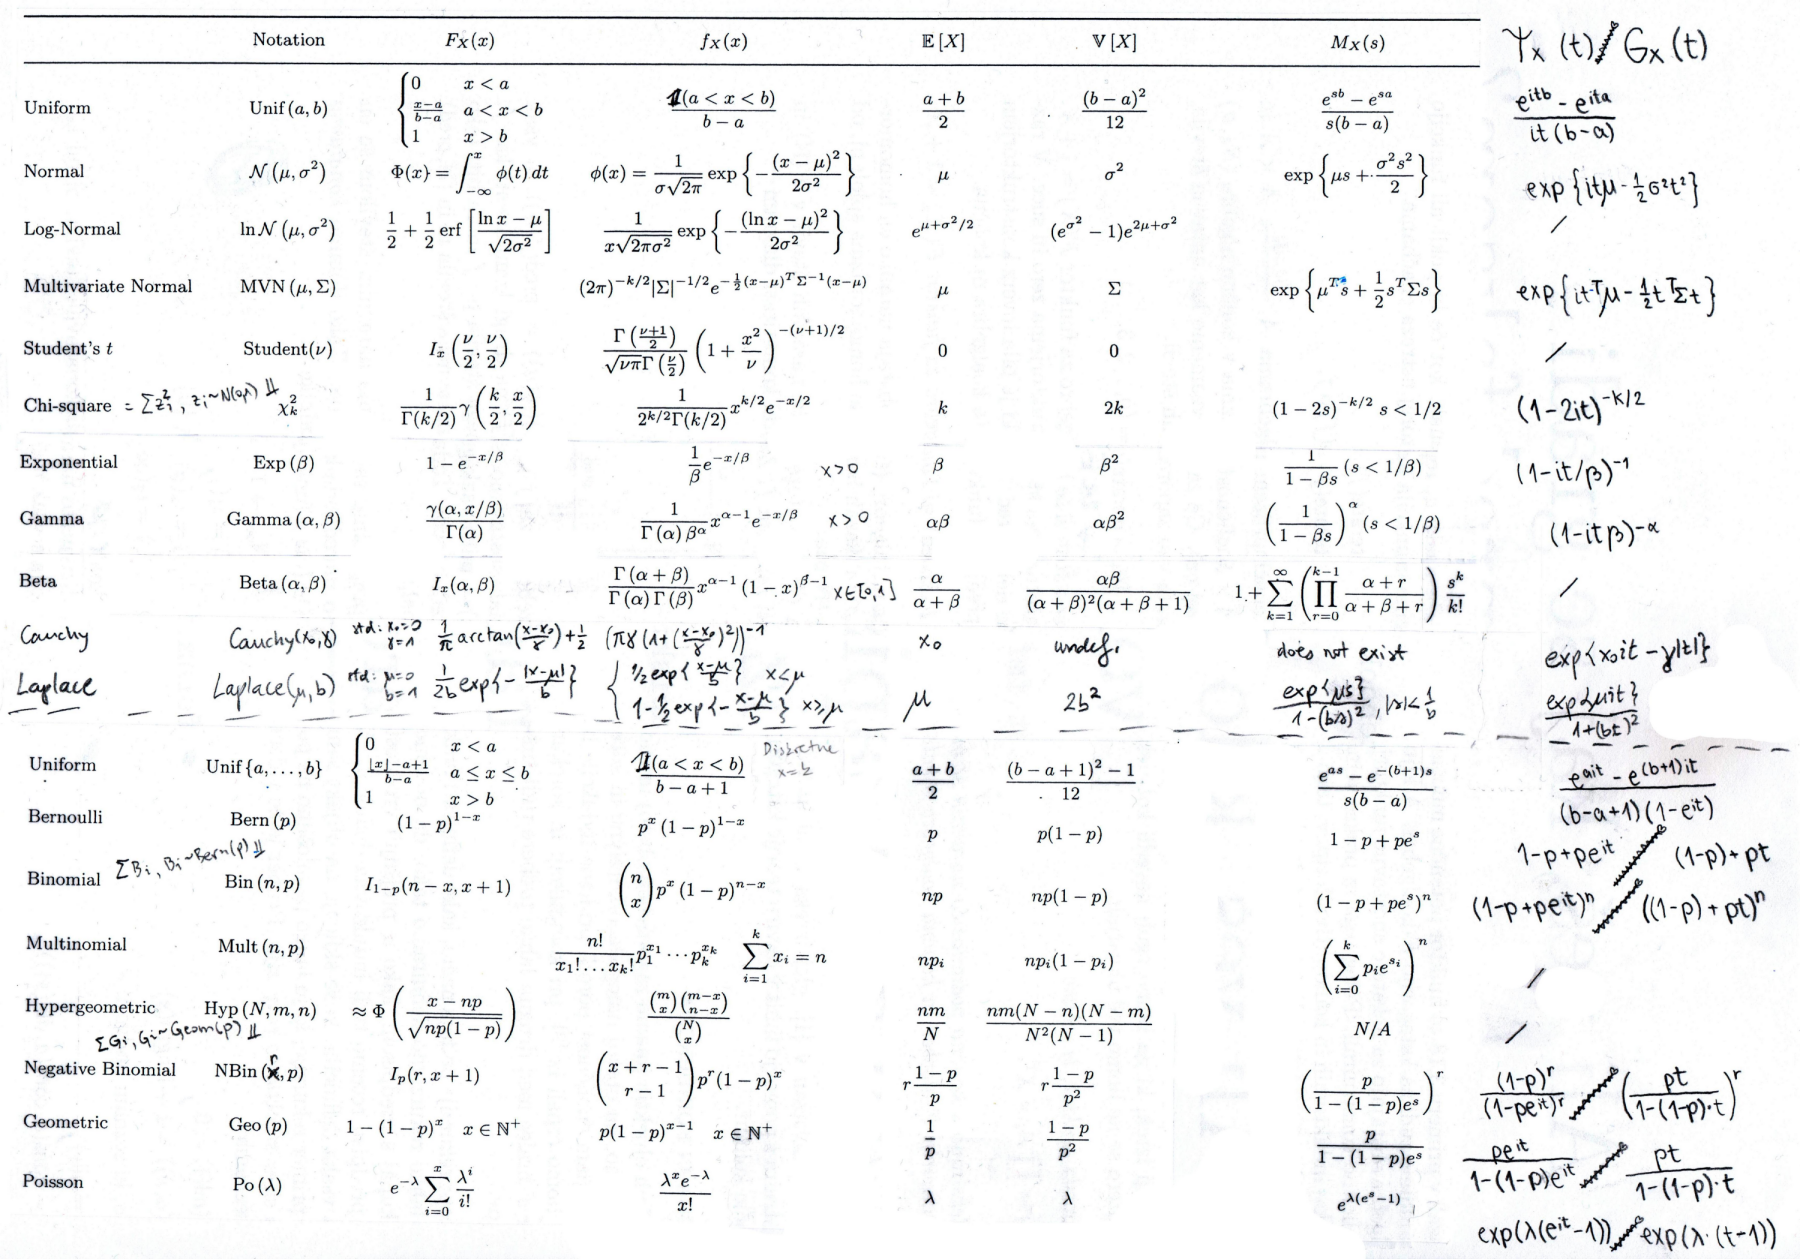
\includegraphics[angle=90,origin=c,width=1\textwidth]{tabela_spremenljivk.png}

\end{document}
